% Created 2016-12-15 Thu 23:24
\documentclass[presentation]{beamer}
\usepackage[utf8x]{inputenc}
\usepackage[T1]{fontenc}
\usepackage{fixltx2e}
\usepackage{graphicx}
\usepackage{longtable}
\usepackage{float}
\usepackage{wrapfig}
\usepackage{rotating}
\usepackage[normalem]{ulem}
\usepackage{amsmath}
\usepackage{textcomp}
\usepackage{marvosym}
\usepackage{wasysym}
\usepackage{amssymb}
\usepackage{hyperref}
\tolerance=1000
\usepackage{minted}
\usetheme{metropolis}
\setbeamertemplate{frame footer}{\color{lightgray}Erwin Rooijakkers - Alliander}
\metroset{block=fill}
\usetheme{default}
\author{Erwin Rooijakkers}
\date{14-12-2016}
\title{Why Clojure?}
\hypersetup{
  pdfkeywords={},
  pdfsubject={},
  pdfcreator={Emacs 25.1.1 (Org mode 8.2.10)}}
\begin{document}

\maketitle

\begin{frame}[label=sec-0-1]{Agenda}
\begin{itemize}
\item Why Clojure is great:
\begin{itemize}
\item It is a Lisp
\item Data-oriented
\item Embraces functional programming
\item JVM + JavaScript runtime
\end{itemize}
\item Demo:
\begin{itemize}
\item Figwheel + Reagent
\end{itemize}
\end{itemize}
\end{frame}

\section{Clojure is a Lisp}
\label{sec-1}

\begin{frame}[label=sec-1-1]{What is so great about Lisp?}
\begin{quotation}
"The most powerful programming language is Lisp. If you don't know Lisp (or its variant, Scheme), you don't know what it means for a programming language to be powerful and elegant. Once you learn Lisp, you will see what is lacking in most other languages." --- Richard Stallman
\end{quotation}
\end{frame}

\begin{frame}[label=sec-1-2]{Parentheses}
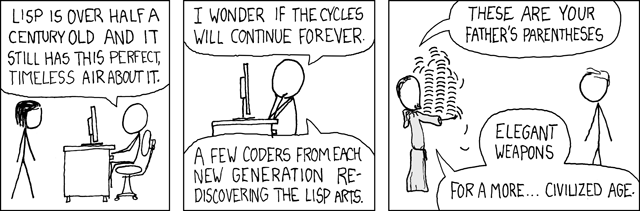
\includegraphics[width=.9\linewidth]{../images/lisp_cycles.png}

(\url{http://xkcd.com/297/})
\end{frame}

\begin{frame}[label=sec-1-3]{Almost all syntax}
\begin{center}
\begin{tabular}{ll}
Lists & \alert{`(1 2 3)}, \alert{`(fred kees piet)}\\
Vectors & \alert{[1 2 3 4 5]}, \alert{[fred kees piet]}\\
Maps & \alert{\{:a 1 :b 2 :b 3\}}, \alert{\{1 kees 2 piet\}}\\
Sets & \alert{\#\{1 2 3\}}\\
Code & \alert{(+ 1 2 3)}  \alert{;; => 6}\\
Naming & \alert{(def n 10)}\\
Lambda & \alert{(def plus-two (fn [a] (+ a *)))}\\
 & \alert{(plus-two 2)} \alert{;; => 4}\\
Quote & \alert{`(+ 1 2 3)} \alert{;; => (+ 1 2 3)}\\
\end{tabular}
\end{center}
\begin{itemize}
\item Parentheses!
\item Code is data and data is code (homoiconicity)
\end{itemize}
\end{frame}

\begin{frame}[fragile,label=sec-1-4]{Parentheses}
 \begin{minted}[bgcolor=white,frame=lines]{clojure}
(+ 1 2 (* 3 4))
\end{minted}
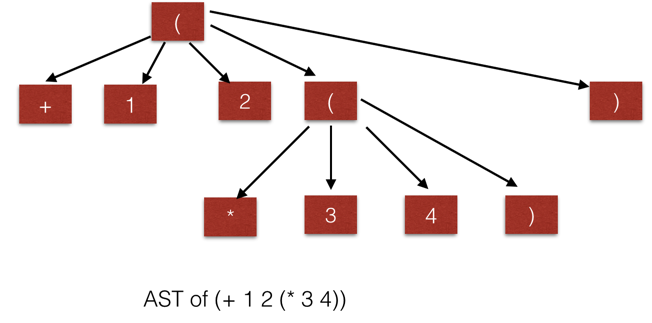
\includegraphics[width=.9\linewidth]{../images/ast.png}
\end{frame}

\begin{frame}[fragile,label=sec-1-5]{Manipulating the AST}
 \begin{minted}[bgcolor=white,frame=lines]{clojure}
(defmacro unless [pred a b]
  `(if (not ~pred) ~a ~b))

;; Usage:
(unless false
 (println "Will print")
 (println "Will not print"))

;; Macro expansion:
(if (not false)
 (println "Will print")
 (println "Will not print"))
\end{minted}
\end{frame}

\begin{frame}[label=sec-1-6]{Programmable programming language}
\begin{itemize}
\item \alert{unless} impossible to implement as function.
\item Second expression is not evaluated!
\item "programmable programming language"
\item Lisp can build any abstraction at all if you can define syntax and semantics for it.
\item Clojure has idiomatic ways of doing that and a small core (no Lisp Curse).
\end{itemize}
\end{frame}

\section{Clojure is data oriented}
\label{sec-2}

\begin{frame}[label=sec-2-1]{Clojure is data oriented}
\begin{quotation}
"It is better to have 100 functions operate on one data structure than 10 functions on 10 data structures." --- Alan Perlis
\end{quotation}
\end{frame}

\begin{frame}[label=sec-2-2]{Clojure is data oriented}
\begin{alertblock}{Rich Hickey time}
\url{https://youtu.be/VSdnJDO-xdg?t=49m8s}
\end{alertblock}
\end{frame}

\section{Clojure embraces functional programming}
\label{sec-3}

\begin{frame}[label=sec-3-1]{Functional programming}
\begin{itemize}
\item End of Moore's law
\item More cores
\item Distributed
\item Parallelism and concurrency
\item How can we adapt our programming practices to this future?
\item Parallelism and concurrency (impossibly) hard in some languages
\end{itemize}
\end{frame}

\begin{frame}[fragile,label=sec-3-2]{Root of the problem}
 \begin{itemize}
\item "\alert{Non-determinism} caused by \alert{concurrent threads} accessing \alert{shared mutable} state."- Martin Odersky
\end{itemize}

\begin{minted}[bgcolor=white,frame=lines]{scala}
var x = 0
async { x = x + 1 }
async { x = x * 2 }
// Can give 0, 1, 2
\end{minted}
(Martin Odersky, "Working Hard to Keep It Simple" - OSCON Java 2011)
\end{frame}

\begin{frame}[label=sec-3-3]{Functional programming}
\begin{itemize}
\item Parallel processing is a fact
\item No mutable state means no problem
\item Imperatively we think in variables and blocks of memory that change over \alert{time}.
\item Functionally we think in \alert{space}: I construct his, then that, then third things out of that.
\item Recursion
\item \alert{Pure functions} are clearer to reason about
\end{itemize}
\end{frame}
\begin{frame}[label=sec-3-4]{Immutable data structures - Structural sharing}
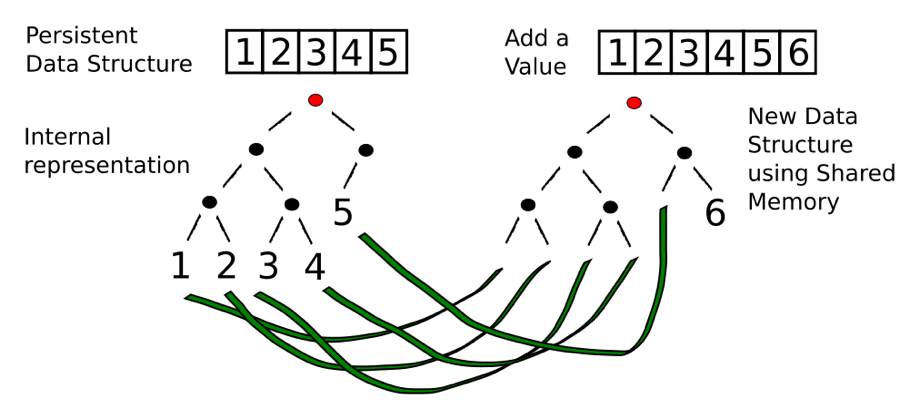
\includegraphics[width=.9\linewidth]{../images/immutable_data_structures.png}
\begin{itemize}
\item Algorithms ensure expected performance characteristics of data structure
\end{itemize}
\end{frame}

\section{Runs on JVM and JavaScript runtime}
\label{sec-4}

\begin{frame}[label=sec-4-1]{JVM and JavaScript}
\begin{itemize}
\item Boring is good.
\item Clojure and ClojureScript embrace host platforms.
\item Sequences implement the expected interfaces.
\item Interop with host.
\end{itemize}
\end{frame}

\begin{frame}[label=sec-4-2]{Demo}
\begin{alertblock}{Figwheel and Reagent}
\ldots{}
\end{alertblock}
\end{frame}

\begin{frame}[label=sec-4-3]{Learn more:}
\begin{itemize}
\item Rich Hickey - Clojure, Made Simple: \url{https://youtu.be/VSdnJDO-xdg}
\item Derek Slager - ClojureScript for Skeptics: \url{https://youtu.be/gsffg5xxFQI}
\item Rich Hickey talks collection: \url{http://bit.ly/1KQNzBr}
\item Bret Victor - Inventing on Principle: \url{https://vimeo.com/36579366}
\end{itemize}
\end{frame}
% Emacs 25.1.1 (Org mode 8.2.10)
\end{document}
